%!xelatex = 'xelatex --halt-on-error %O %S'

\documentclass{buaaemp}
\begin{document}

% 标题,作者
\emptitle{单色仪}
\empauthor{智朝晖}{蔡微}

% 奇数页页眉 % 请在这里写出第一作者以及论文题目
\fancyhead[CO]{{\footnotesize 智朝晖: 单色仪}}


%%%%%%%%%%%%%%%%%%%%%%%%%%%%%%%%%%%%%%%%%%%%%%%%%%%%%%%%%%%%%%%%
% 关键词 摘要 首页脚注
%%%%%%%%关键词
\Keyword{单色仪, 钠黄双线,吸收曲线,吸收系数}
\twocolumn[
\begin{@twocolumnfalse}
\maketitle

%%%%%%%%摘要
\begin{empAbstract}
单色仪是指能把宽波段的电磁辐射分离为一系列狭窄波段的电磁辐射的仪器。本实验利用单色仪进行了钠黄光灯的光谱线的测量并且测量了得到钕玻璃在550.0nm到620.0nm范围的吸收谱曲线以及吸收系数曲线。
\end{empAbstract}

%%%%%%%%首页角注,依次为实验时间、报告时间、学号、email
\empfirstfoot{2022-11-10}{2022-11-10}{20377365}{20377365@buaa.edu.cn}
\end{@twocolumnfalse}
]
%%%%%%%%!首页角注可能与正文重叠,请通过调整正文中第一页的\enlargethispage{-3.3cm}位置手动校准正文底部位置:
%%%%%%%%%%%%%%%%%%%%%%%%%%%%%%%%%%%%%%%%%%%%%%%%%%%%%%%%%%%%%%%%
%  正文由此开始
\wuhao 
%  分栏开始

\section{引~~言}
单色仪是指能把宽波段的电磁辐射分离为一系列狭窄波段的电磁辐射的仪器。常见的有棱镜单色仪和光栅单色仪两种。光栅单色仪利用光栅衍射的方法吧紫外光可见光红外光分解为单色光。单色仪是一种常用的分光仪器,利用色散元件把复色光分解为准单色光,能输出一
系列独立的、光谱区间足够窄的单色光,可用于各种光谱分析和光谱特性的研究,如测
量介质的光谱透射率曲线、光源的光谱能量分布、光电探测器的光谱响应等,应用相当
广泛。

光栅单色仪是把复合光分解为一系列高纯度的单色光的仪器。仪器具有波长范围宽、
分辨本领高、波长精度高、扫描速度调节范围大等特点。主要用于物质的定量和定性分
析、光源特性、溶液的浓度、光的生效效应和透明物质的光学特性等研究工作。自动化
程度高(能自动扫描光谱,自动滤波光片),可用于测各种辐射源的光谱分布、探测器
的光谱灵敏度、发光材料及光学薄膜的光谱特性等等。它可广泛地用于化学、制药、造
纸、建筑、材料、仪器仪表、环境保护、光学真空镀膜等方面。
与棱镜单色仪不同,光栅单色仪是通过衍射来实现复色光的分解的。光栅光谱仪是多种多样的,其主要是由光
栅、狭缝、成像系统和感光板(或出射狭缝)等部件组成。光栅单色仪与棱镜单色仪最大
的不同主要是在光学系统上。如图 \ref{fig:my_label1}所示,这是一种平面光栅单色仪的光学系统结构示意图。

\newpage

它的工作原理是光源发出的光均匀的照亮在位于抛物镜的焦平面上的狭缝 S1,然后经过凹面镜 M1 的反射到光栅 G 上。由光栅的衍射光再经过 M1、M2 的反射后射出狭缝 S2。
相比于棱镜单色仪来说,光栅单色仪由于没有太多折射,光强减少相对较小,出射光强较大。因此光栅单色仪比较容易与其它检测设备配套使用。而且由于光栅相对于棱镜来
说体积较小,并且光栅制作技术的不断进步,现在光栅单色仪的应用更加广泛。因此,
光栅单色仪的分类也就比较多了。它们的结构大多是保持入射狭缝和出射狭缝不动,仅
光栅自身转动来实现谱线的扫描和波长的选择。
现在,众多的光谱仪谱线的观测一般也不再是凭肉眼观察,而是利用光电倍增管、
线阵 CCD 等高灵敏光电转换器件,不仅可以观察谱线位置,而且可以精确测量各波长处
的光谱强度;其棱镜或光栅的转动也利用步进装置实现自动精确的转动,在计算机的控
制下自动实现调节、测量和分析。
\cite{钱建强2016近代物理实验}

\section{原~~理}
\subsection{光栅方程}
设有一束光以入射角$  q_{0}$  射向一块衍射光栅, 则只有满足下式的一些特殊 角度 $ q_{m}$  下, 才有光束衍射出来: $ d\left(\sin \theta_{0} \pm \sin \theta_{m}\right)=m \lambda $
\subsection{强度分布}
光栅方程只说明了各级衍射的衍射方向, 按照多缝衍射的理论, 在强度. 为  $I_{0}$  的入射光照射下, 光栅衍射光的强度分布为:

\begin{equation}
    I=I_{0} A(\mu) \cdot B(v)=I_{0} \frac{\sin ^{2} \mu}{\mu^{2}} \cdot \frac{\sin ^{2}(N v)}{N^{2} \sin ^{2} v}
\end{equation}


\subsection{光栅的角色散}
从光栅方程可以得到光栅的角色散为:  $\frac{d \theta_{m}}{d \lambda}=\frac{m}{d \cos \theta_{m}} $ 当衍射角较小 时  $\operatorname{cosqm} \approx 1$ , 则式子可变为:  $\frac{d \theta_{m}}{d \lambda}=\frac{m}{d} $
 
 \subsection{光栅的分辨率}
 $ \frac{\Delta \lambda}{\lambda}=(N \times m)^{-1}  $为进一步说明光栅的分辨率和各种因素的关系, 利用光栅方程, 得  
 \begin{equation}
     \frac{\lambda}{\Delta \lambda}=\frac{W}{\lambda}\left(\sin \theta_{0}+\sin \theta_{m}\right) 
 \end{equation}

\subsection{吸收曲线测量原理}

当光束入射到有定厚度的介质平板上时, 有一部分光被反 射,另一部分光被介质吸收, 剩下的光从介质板透射出来。设有一束波长为 $ \lambda$ , 入射光 强为  $\mathrm{I}_{0}$  的单色平行光垂直入射到一块厚度为 $ \mathrm{d}$  的介质平板上, 定义介质板的光谱外透射 率  $\mathrm{T} $ 和介质的光谱透射率 $ \mathrm{Ti}$  分别为: $ T=\frac{I_{T}}{I_{0}} \quad T_{i}=\frac{I_{2}}{l_{1}} $ 设光在单一界面上的反射率为 $ \mathrm{R} $ ,则 透射光的光强为 $ I_{T}=\frac{I_{0}(1-R)^{2} e^{-\alpha d}}{1-R^{2} e^{-2 a d}}  所以  T=\frac{I_{T}}{I_{0}}=\frac{\left.(1-R)^{2} e^{-\alpha d}\right)}{\left.1-R^{2} e^{-2 a d}\right)}$  设两块试样的厚度分别 
$d_1$,$d_2$,则 $\frac{T_2}{T_1}=e^{\alpha (d_2-d_1)}$,所以
\begin{equation}
    \alpha=\frac{lnT_2-lnT_1}{d_2-d_1}
\end{equation}

合适的条件下, 单色仪测量输出的数值与照射到它的光的强度成正比。
所以读出测量 的强度就可由下式计算光谱透射率和吸收系数:
\begin{equation}
    T_i=\frac{I_2}{I_1}
\end{equation}

\begin{equation}
    \alpha=\frac{ln(I_2 / I_1)}{d_2-d_1}
\end{equation}

\begin{figure}
    \centering
    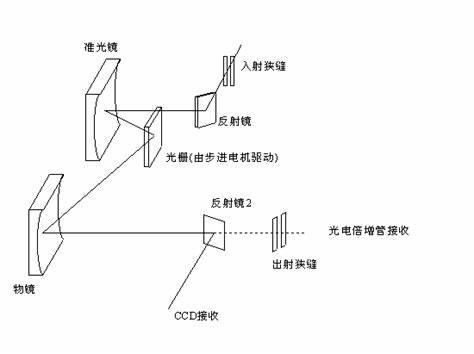
\includegraphics[width=\linewidth]{image/OIP-C.jpg}
    \caption{闪耀光栅单色仪内部结构}
    \label{fig:my_label1}
\end{figure}
\section{实~~验}
本实验利用WDP500-C型单色仪进行了钠黄光灯的光谱线的测量,同时利用WDPF-C测光仪测光强得到了钠双黄线的位置并且测量了钕玻璃在550.0nm到620.0nm范围的吸收谱曲线。

先将单色仪的波长定在589-591nm之间的某个数,将出射缝 $S_2$宽度调到2mm左右。用眼睛迎着出射光方向观察 调节$S_1$的宽度$S_2$上钠的两条黄色谱线(589.0nm, 589.6nm)分开为止,在调节 $S_2$的宽度使得$S_2$的宽度与任一条黄谱线的衍射像宽度大致相等,此时开始测量从589nm-591nm范围内的钠黄光光强。

测完后换用溴钨灯作为光源,此光源光谱线较为平缓,方法同前。在入射缝装上钕玻璃,观察光电倍增管连接的测光仪读数。
\section{实验结果与分析}
得到实验数据如下:
\begin{array}{|l|l|l|l|}
\hline \text { 波长 } / \mathrm{nm} & \text { 示数 } & \text { 波长 } / \mathrm{nm} & \text { 示数 } \\
\hline 587.7 & 1 & 589.9 & 
165 \\
\hline 587.8 & 1 & 590.0 & 
264 \\
\hline 587.9 & 2 & 590.1 & 
290 \\
\hline 588.0 & 3 & 590.2 & 
200 \\
\hline 588.1 & 4 & 590.3 & 
157 \\
\hline 588.2 & 4 & 590.4 & 
145 \\
\hline 588.3 & 4 & 590.5 & 
150 \\
\hline 588.4 & 4 & 590.6 & 
160 \\
\hline 588.5 & 5 & 590.7 & 
180 \\
\hline 588.6 & 7 & 590.8 & 
124 \\
\hline 588.7 & 11 & 590.9 & 64 \\
\hline 588.8 & 13 & 591.0 & 52 \\
\hline 588.9 & 15 & 591.1 & 43 \\
\hline 589.0 & 17 & 591.2 & 33 \\
\hline 589.1 & 17 & 591.3 & 27 \\
\hline 589.2 & 20 & 591.4 & 20 \\
\hline 589.3 & 27 & 591.5 & 16 \\
\hline 589.4 & 50 & 591.6 & 14 \\
\hline 589.5 & 81 & 591.7 & 13 \\
\hline 589.6 & 112 & 591.8 
& 10 \\
\hline 589.7 & 120 & 591.9 
& 8 \\
\hline 589.8 & 130 & 592.0 
& 5 \\
\hline
\end{array}

\begin{array}{|l|l|l|l|l|}
\hline \multicolumn{2}{|l|}{\mathrm{d} 1=1.80 \mathrm{~mm}} & \multicolumn{2}{l|}{\mathrm{d} 2=1.27 \mathrm{~mm}} & \\
\hline \text { 波长 } / \mathrm{nm} & \text { 示数 } & \text { 波长 } / \mathrm{nm} & \text { 示数 } & \text { 吸收系数 } \\
\hline 550 & 40 & 550 & 38 
& 0.09678 \\
\hline 555 & 42 & 555 & 40 
& 0.092057 \\
\hline 560 & 42 & 560 & 41 
& 0.045467 \\
\hline 565 & 43 & 565 & 40 
& 0.136454 \\
\hline 570 & 33 & 570 & 16 
& 1.365885 \\
\hline 575 & 23 & 575 & 9 & 1.77032 \\
\hline 580 & 20 & 580 & 7 & 1.980796 \\
\hline 581 & 19 & 581 & 7 & 1.884017 \\
\hline 582 & 18 & 582 & 7 & 1.782003 \\
\hline 583 & 17 & 583 & 5 & 2.30901 \\
\hline 584 & 17 & 584 & 4 & 2.730036 \\
\hline 585 & 17 & 585 & 3 & 3.272832 \\
\hline 586 & 20 & 586 & 2 & 4.3445 \\
\hline 587 & 22 & 587 & 2 & 4.524331 \\
\hline 588 & 25 & 588 & 3 & 4.000497 \\
\hline 589 & 26 & 589 & 4 & 3.531702 \\
\hline 590 & 29 & 590 & 4 & 3.737739 \\
\hline 591 & 32 & 591 & 5 & 3.502449 \\
\hline 592 & 33 & 592 & 5 & 3.560509 \\
\hline 593 & 35 & 593 & 6 & 3.327526 \\
\hline 594 & 36 & 594 & 7 & 3.089828 \\
\hline 595 & 37 & 595 & 9 & 2.667346 \\
\hline 600 & 46 & 600 & 23 
& 1.307825 \\
\hline 605 & 48 & 605 & 35 
& 0.595949 \\
\hline 610 & 50 & 610 & 42 
& 0.328969 \\
\hline 615 & 52 & 615 & 51 
& 0.036638 \\
\hline 620 & 50 & 620 & 49 
& 0.038118 \\
\hline
\end{array}

处理数据后得到图像如下:
\begin{figure}
    \centering
    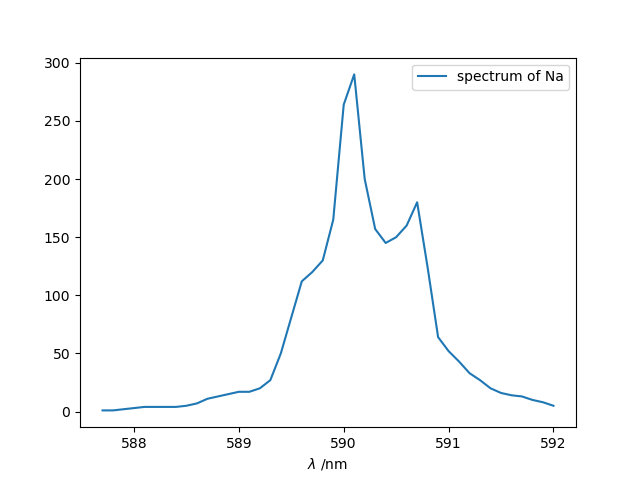
\includegraphics[width=\linewidth]{image/spectrum.png}
    \caption{Na元素的光谱}
    \label{fig:my_label2}
\end{figure}
\begin{figure}
    \centering
    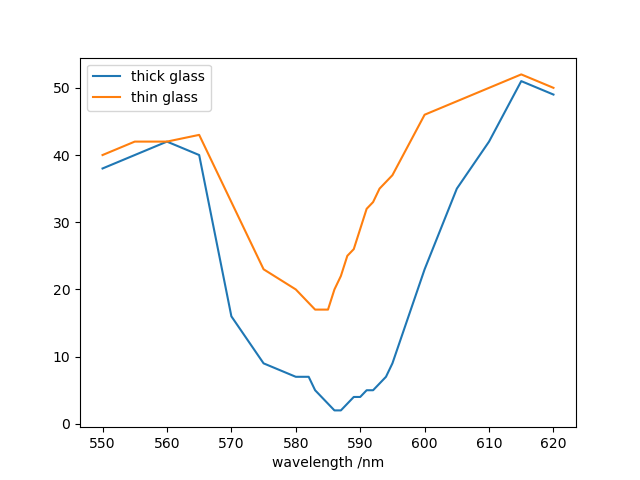
\includegraphics[width=\linewidth]{image/absorption.png}
    \caption{钕玻璃的吸收曲线}
    \label{fig:my_label3}
\end{figure}

\begin{figure}
    \centering
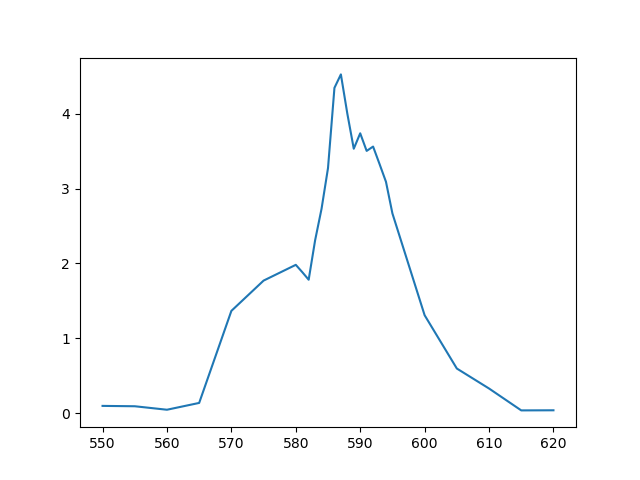
\includegraphics[width=\linewidth]{image/absorptioncoeff.png}
    \caption{钕玻璃的吸收系数曲线}
    \label{fig:my_label4}
\end{figure}

\section{思考题}
\begin{itemize}
    \item 使入射光能照明整个光栅,以便有尽量多的光从出射狭缝射出。
    \item 校对单色仪波长示值时应当采用有确定辐射可见谱线的光源,汞灯在可见光谱内有确定的579.1nm、 577.0nm、546.1nm、435.8nm 的可见谱线。测量吸收曲线则应该尽量选择在谱线范围内光强平稳的光源,比如溴钨灯。
    \item 出射光狭缝宽度与入射光狭缝都与谱线宽度成正比关系,入射狭缝的宽度越小则出射光的单色性越好,出射狭缝的宽度与出射光的单色性。
    \item 因为我们测量吸收曲线是在不同玻璃片厚度测量相同波长的光的吸收效果,此时光电倍增管的光谱响应效应相同。
\end{itemize}
\section{结~~论}
本实验利用单色仪进行了钠黄光灯的光谱线的测量,得到了钠双黄线的位置,可以看到分别在590.1nm和590.7nm,测得的双黄线波长差与已知数据一致,说明我们的实验操作基本无误,但是双峰的位置偏差了1.1nm说明可能是实验仪器的误差问题。并且我们测量了钕玻璃在550.0nm到620.0nm范围的吸收谱曲线,可以看到吸收峰在585nm-595nm之间,说明钕玻璃在这个区间内吸收效果最好。


%%%%%%%%%%%%%%%%%%%%%%%%%%%%%%%%%%%%%%%%%%%%%%%%%%%%%%%%%%%%%%%%
%  参考文献
%%%%%%%%%%%%%%%%%%%%%%%%%%%%%%%%%%%%%%%%%%%%%%%%%%%%%%%%%%%%%%%%
%  参考文献按GB/T 7714-2015《文后参考文献著录规则》的要求著录. 
%  参考文献在正文中的引用方法:\cite{bib文件条目的第一行}

\renewcommand\refname{\heiti\wuhao\centerline{参考文献}\global\def\refname{参考文献}}
\vskip 12pt

\let\OLDthebibliography\thebibliography
\renewcommand\thebibliography[1]{
  \OLDthebibliography{#1}
  \setlength{\parskip}{0pt}
  \setlength{\itemsep}{0pt plus 0.3ex}
}

{
\renewcommand{\baselinestretch}{0.9}
\liuhao
\bibliographystyle{gbt7714-numerical}
\bibliography{./TempExample}
}


\end{document}
